



% -------------------------------------------------------------------------
% Section: Modeling the Variability Mechanisms
% ------------------------------------------------------------------------
\section{SVCM Approach}
\label{sec:models}

To solve the problems mentioned in the previous section, we introduce now our
approach for modeling variabilities in use case scenarios, which was named as
\emph{Scenario Variability as Crosscutting Mechanisms} (SVCM). It improves the
separation of concerns between variability management and scenario specifications, dealing with scenario variability as a composition of the
following artifacts: SPL use case model, feature model, product configuration,
and configuration knowledge. 

Motivated by the Masuhara and Kiczales
framework~\cite{Masuhara:2003aa}, our approach for \textbf{scenario variability
management} is based on a weaving process that takes as input the aforementioned
specifications, which crosscut each other with respect to the resulting product
specific use case model (Figure~\ref{fig:weave-process}). Combining these input
languages, it is possible to represent the sources of variability that we are
interested in: \emph{variation in function}, \emph{variation in data}, and
\emph{variation in control flow}~\cite{Bachmann:2001aa}.

\textcolor{red}{
We detail our approach showing how it
can be used to specify the motivating example... 
after that we describe the semantics of our approach using a slight
customization of the MK...
}

\subsection{SVCM example}
\label{sub:running}

In order to explain how the input models (Figure~\ref{fig:weave-process})
crosscut each other with respect to the final product, in this section we
present a running example of our approach. Several artifacts of each input model
are shown; mentioning the contribution of these models to the whole weaving
process.

\subsubsection{Feature model}

Feature models have an important contribution to our
weaving process, since they are used for checking if a product
configuration is a valid member of the product line. It is important to note
that we are not proposing a new notation for feature modeling. Here we
only present the features required (Figure~\ref{fig:eshop-fm-re}) for
understanding the SVCM example.

\begin{figure}[h]
 \begin{center}
  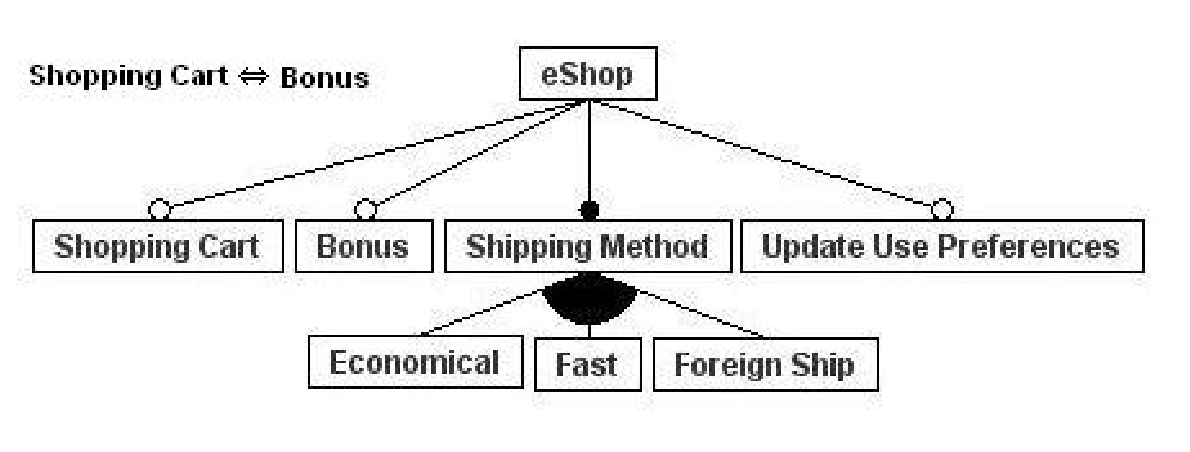
\includegraphics[scale=0.40]{img/eShop-FM2.eps}
   \caption{Subset of eShop feature model.}
  \label{fig:eshop-fm-re}
  \end{center}
\end{figure}

Based on the feature model of Figure~\ref{fig:eshop-fm-re}, the \emph{Shopping
Cart}, \emph{Bonus} and \emph{Update User Preferences} features are optional; on
the other hand, the \emph{Shipping Method} feature is mandatory and all products
have to be configured with at least one of its child. Additionally, the
restriction $Shopping\ Cart\ \Leftrightarrow\ Bonus$ states that all
products configured with the shopping cart feature must also be configured with
the bonus feature. More details about feature modeling can be found
elsewhere~\cite{Gheyi:2006aa,Czarnecki:2000aa}.


\subsubsection{SPL use case model}

This artifact defines scenarios that describe the expected behavior of the SPL's
members. Scenarios might be optional, have parameters, and change (advice) the
behavior of other scenarios. A use case model is composed by \emph{use cases} and
\emph{aspectual use cases}. A use case has a name, a description and a list of
scenarios, which consist of a sequence of steps (pairs of \emph{User action x
System response}). An aspectual use case has a name and a list of advice, which
can be used to extend the behavior of existing scenarios. Differently from
PLUSS and PLUC, our proposed scenarios are not enriched with alternative steps,
product definition, and information related to configurability.  

In this SVMC example, we consider the following scenarios and advices:

{\bf Proceed to Purchase:} this mandatory scenario
(Figure~\ref{fig:proceed-to-checkout}) specifies the common behavior that is
required for confirming a purchase. Instances of the product line must be
configured with this scenario. Notice that a parameter
\emph{ShippingMethod} is referenced in Step P2. This parameter (notation
also supported in PLUSS and PLUC) allows the reuse of the \emph{Proceed to
Purchase} scenario for different configurations of \emph{shipping method}. 

\begin{figure}[h]
\begin{scriptsize}
  \texttt{
   \begin{tabular}{l}
   	 {\bf Id: SC01} 	\\
     {\bf Description:} Proceed to purchase\\
   \end{tabular}
  \begin{center}
  \begin{tabular}{||p{0.1in}||p{1.4in}||p{1.4in}||}
   \hline
       Id & User Action  & System Response \\ \hline \hline
       P1 & Fill in the requested information and select the proceed option.  & Request the shipping method and address.\\  \hline
       P2 & Select one of the available ship methods (\mbox{<ShippingMethod>}),
       fill in the destination address and proceed. & Calculate the shipping costs. \\  \hline P3 & Confirm the purchase. & Execute the order and send a request to the Delivery System to dispatch the products.
       \mbox{[RegisterPreference]} \\  \hline
  \end{tabular}
  \end{center}
  }
\end{scriptsize}
\caption{Proceed to purchase scenario.}
\label{fig:proceed-to-checkout}
\end{figure}

{\bf Buy Product:} this advice (Figure~\ref{fig:buy-product-scenario}) enables a
customer to buy specific goods from an online shopping store. It is only
available in the product line members that are {\bf not} configured with the
\emph{Shopping Cart} and \emph{Bonus} features. Differently from the PLUSS
approach, which directly relates alternative and optional steps to features, in
our approach this kind of information is represented in a distinct artifact: the
configuration knowledge. The effect of this advice is to introduce an optional behavior {\bf
before} the join points identified in its \emph{pointcut} clause. In this case,
the Step P1 defined in the \emph{Proceed to Purchase} scenario.

\begin{figure}[h]
\begin{scriptsize}
  \texttt{
   \begin{tabular}{l}
   	 {\bf Id: ADV01} 	\\
     {\bf Description:} Buy a specific product\\
     {\bf Before:}  P1
   \end{tabular}
  \begin{center}
  \begin{tabular}{||p{0.1in}||p{1.4in}||p{1.4in}||}
   \hline
       Id & User Action  & System Response \\ \hline \hline
       B1 & Select the buy product option.  & Present the selected product. The user can change the quantity of items he wants to buy. Calculate and show the amount to be paid. \\  \hline
       B2 & Select the confirm option. &  Request payment information. \\  \hline
    \end{tabular}
  \end{center}
  }
\end{scriptsize}
\caption{Buy product advice.}
\label{fig:buy-product-scenario}
\end{figure}

{\bf Buy Products with Shopping Cart and Bonus:} this advice
(Figure~\ref{fig:buy-product-changing-flow}) allows purchasing products
that have been previously added to a customer shopping cart. It extends the
behavior of the \emph{Proceed to Purchase} scenario by introducing the specific
behavior required by the \emph{Shopping Cart} and
\emph{Bonus} features. Therefore, this advice is required by products that
are configured with both \emph{Shopping Cart} and \emph{Bonus} features.

\begin{figure}[h]
\begin{scriptsize}
  \texttt{
   \begin{tabular}{l}
   	 {\bf Id: ADV02} 	\\
     {\bf Description:} Buy products using a shopping-cart\\
     {\bf Before:} P1
   \end{tabular}
  \begin{center}
   \begin{tabular}{||p{0.1in}||p{1.4in}||p{1.4in}||}
   \hline
       Id & User Action & System Response \\ \hline \hline
       C1 & Select the checkout option.  & Present the items in the shopping cart and the amount to be paid. The user can remove items from the shopping cart. \\  \hline
       C2 & Select the confirm option. & Request bonus and payment information. \\  \hline
  \end{tabular}
  \end{center}
  }
\end{scriptsize}
\caption{Buy products with shopping cart advice.}
\label{fig:buy-product-changing-flow}
\end{figure}

As shown in Section~\ref{sec:problem}, PLUSS and PLUC represent all valid
configurations of a scenario in a single artifact. Using our approach, we were
able to separate the common behavior required to confirm a purchase (the base
scenario \emph{Proceed to Purchase}) from its variants, specified in the
\emph{Buy Product} and \emph{Buy Product with Shopping Cart} advices. This allows
our specifications to evolve according to the \emph{Open-Closed}
principle~\cite{Meyer:2000aa}. In our approach, introducing new product
variants require more extensions than changes to the base scenarios.



{\bf Search for Products:} this mandatory scenario
(Figure~\ref{fig:search-products-flow}) allows the user to search for products.
In order to save space, we only present Step S3, which performs a search based
on the input criteria. This step is annotated with the mark \mbox{{\bf [RegisterPreference]}}, exposing
it as a possible extension point for the behavior of \emph{Register User
Preferences} (Figure~\ref{fig:register-preferences-flow}). The same annotation
was assigned to the Step P3 of \emph{Proceed to Purchase}
(Figure~\ref{fig:proceed-to-checkout}). Such annotations can be referenced by advices, 
and were proposed as an attempt to reduce the problem of fragile pointcuts.
\textcolor{red}{We believe that introducing semantic based mechanisms to compose
scenarios~\cite{Chitchyan:2007aa} does not require significant changes to
the SVMC weaving process.}  

\begin{figure}[ht]
\begin{scriptsize}
  \texttt{
   \begin{tabular}{l}
   	 {\bf Id: SC02} 						\\
     {\bf Description:} Search for products. \\
   \end{tabular}
  \begin{center}
   \begin{tabular}{||p{0.1in}||p{1.4in}||p{1.4in}||}
   \hline
       Id & User Action &  System Response \\ \hline \hline
       \ldots & \ldots  & \ldots \\  \hline
       S3 & Inform the search criteria. &  Retrieve the products that satisfy the search criteria. Show a list with the resulting products. [RegisterPreference] \\  \hline
  \end{tabular}
  \end{center}
  }
\end{scriptsize}
\caption{Search for products scenario.}
\label{fig:search-products-flow}
\end{figure}

{\bf Register User Preferences:} this advice updates the user preferences based
on the user's history of searches and purchases. Its behavior can be started {\bf
after} any step assigned to the {\bf [RegisterPreference]} (see the
\emph{pointcut} clause) annotation and is available in products that are
configured with the \emph{Update User Preferences} feature.

\begin{figure}[h]
\begin{scriptsize}
  \texttt{
   \begin{tabular}{l}
   	 {\bf Id: ADV03} 	\\
     {\bf Description:} Register user preferences.\\
     {\bf After}: [RegisterPreference] \\
   \end{tabular}
  \begin{center}
   \begin{tabular}{||p{0.1in}||p{1.4in}||p{1.4in}||}
   \hline
       Id & User Action &  System Response \\ \hline \hline
       R1 & - &  Update the preferences based on the search results or purchased items. \\  \hline
  \end{tabular}
  \end{center}
  }
\end{scriptsize}
\caption{Register user preferences.}
\label{fig:register-preferences-flow}
\end{figure}

In this example, we described several scenarios as being optional or
mandatory. It is important to observe that, in our approach, this kind of
information is not specified in scenario documents. Actually, it is necessary to
consider the relationships between scenarios and features in order to realize
which configurations require a specific scenario. As we explained at the
beginning of this section, each artifact (feature model, product configuration,
configuration knowledge, and use case model) provides a specific contribution to
the definition of a SPL's member.


\subsubsection{Product configuration}\label{subsub:pc}

This artifact identifies a SPL member, which is characterized by a valid
configuration of features. Each product configuration should conform to a
feature model (the selected features should obey the feature model relationships and constraints). Two possible configurations are presented in
Figure~\ref{fig:product-config-01-02}. We represent these configurations as a
tree, highlighting which features were selected. Such a representation was
created using the \emph{Feature Modeling Plugin}~\cite{czarnecki-eclipse-2004}

 \begin{figure}[h]
 \begin{center}
  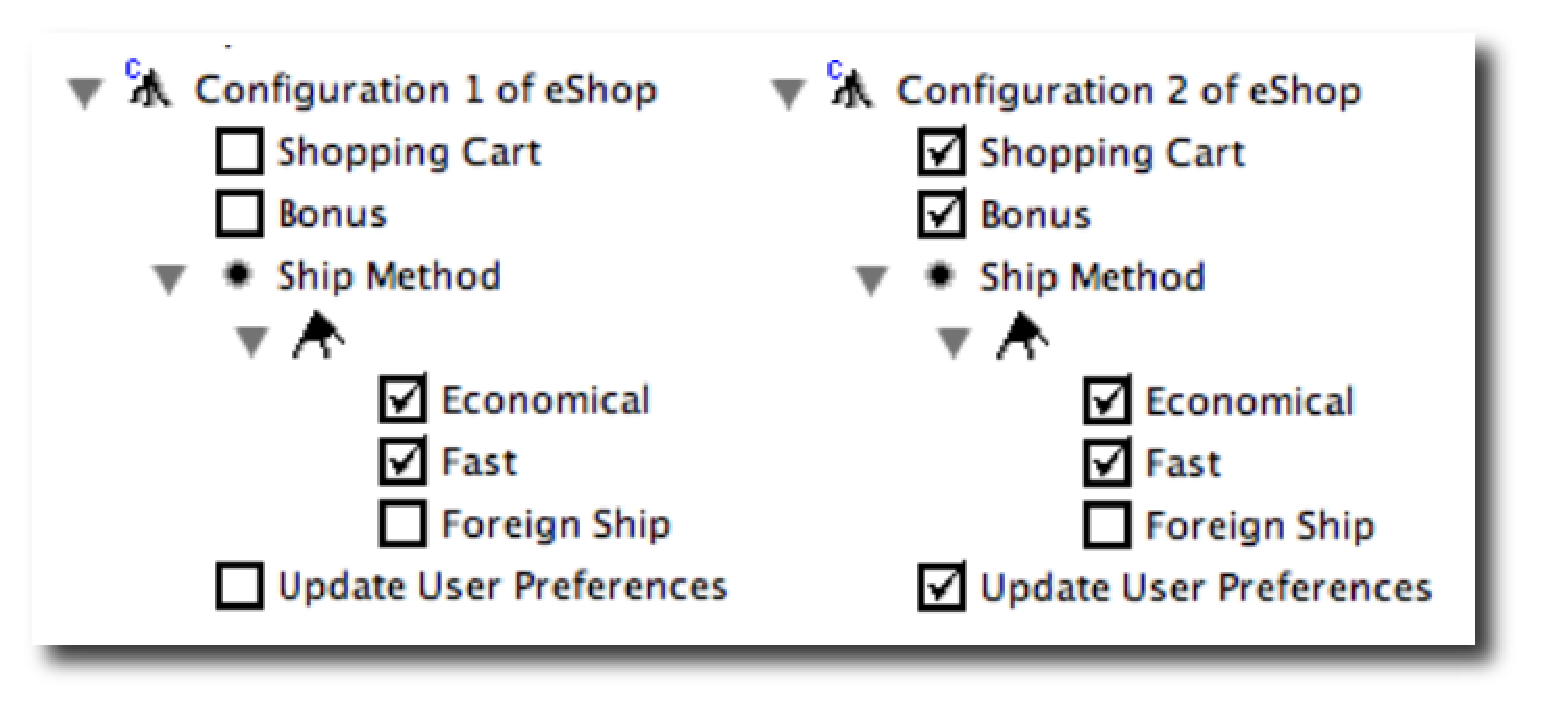
\includegraphics[scale=0.33]{img/pc-04.eps}
   \caption{Examples of product configurations.}
  \label{fig:product-config-01-02}
  \end{center}
\end{figure}

% \begin{figure}[htb] \centerline{
% \mbox{
\includegraphics[scale=0.4]{img/pc-01.eps}}
% \mbox{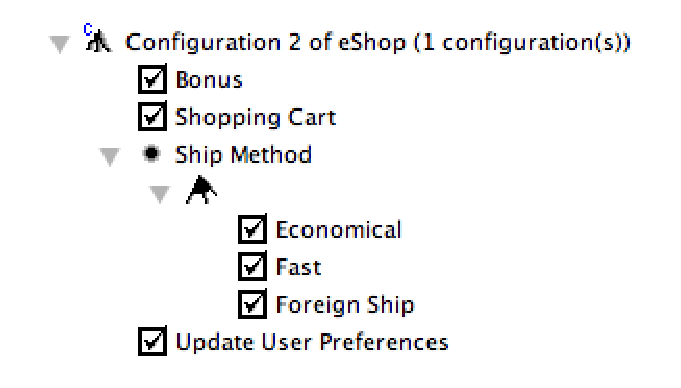
\includegraphics[scale=0.4]{img/pc-02.eps}} } \nocaptionrule
% \caption{Examples of product configurations.} \label{fig:product-config-01-02}
% \end{figure}

The first configuration (on the left side of the
Figure~\ref{fig:product-config-01-02}) defines a product that has no support for
\emph{shopping cart}, \emph{bonus} and \emph{preferences update}. Additionally,
it supports only the economical and fast ship methods. The second configuration
is more complete, being configured with the features \emph{shopping cart},
\emph{bonus}, and \emph{update user preferences}.

\subsubsection{Configuration knowledge}

This artifact is represented as a list of configuration items, which relates
feature expressions to weavers (Figure~\ref{fig:wp-semantics}). Since these
weavers are responsible for generating specific instances of a SPL,
the configuration knowledge allows, during product engineering, the automatic
configuration of SPL assets. Figure~\ref{fig:ck-running-example} presents the
configuration knowledge ($ck$) for the running example, enforcing that:

\begin{itemize}
\item Both \emph{Proceed to Purchase} (SC01) and \emph{Search for Products}
(SC02) scenarios are mandatory, since their selection is related to the
(mandatory) root feature of \emph{eShop} product line;

\item The \emph{Buy Product} advice (ADV01) is used in the composition of
products that do not have been configured with both \emph{Shopping Cart} and \emph{Bonus}
features --- if both features were selected for a product, it would be configured
with the \emph{Buy Product with Cart} advice (ADV02);

\item The \emph{Register User Preferences} advice (ADV03) is not used in a
product composition unless the \emph{Update User Preferences} feature has been
selected; and

\item References to the ``ShipMethod'' parameter are bound to the
selected alternatives of \emph{Ship Method} feature.

\end{itemize}

\begin{figure*}[hbt]
 \begin{code}
  (|->) :: a -> b -> (a,b) -- just a 'syntactic sugar' to build pairs
  l |-> r = (l,r)

  conf1 = Configuration (``eShop'' |-> selectScenarios[``SC01'', ``SC02''])
  conf2 = Configuration ('Not' (``ShoppingCart'' 'And' ``Bonus'') |-> evaluateAdvice[``ADV01''])
  conf3 = Configuration (``ShoppingCart'' 'And' ``Bonus'' |-> evaluateAdvice[``ADV02''])
  conf4 = Configuration (``UpdateUserPreferences'' |-> evaluateAdvice[``ADV03''])
  conf5 = Configuration (``ShipMethod'' |-> bindParameter(``ShipMethod'', `ShipMethod''))
  ...

  ck = [conf1, conf2, conf3, conf4, conf5]
 \end{code}
\caption{eShop configuration knowledge}
\label{fig:ck-running-example}
\end{figure*}

We can reason about the effect of evaluating a configuration knowledge
by means of trace models, defined to our context as:

\newdef{definition}{Definition}

\begin{definition}
A trace model is the set of valid sequences of events
computed from the product scenarios. Events are labeled as the step ids of a
scenario. The trace model for a scenario $s$ is given by:.
\end{definition}

\begin{code}
traceModel s = traces (steps s)
where
  traces [] = [[]]
  traces (x:xs) = [] : (stepId x) ^ (traces (xs))

(^) :: (a -> [[a]]) -> [[a]]
x ^ y = [ x:e | e <- y ]
\end{code}

For instance, Table~\ref{tab:ck-evaluation} presents the resulting trace models,
after evaluating each configuration item of Figure~\ref{fig:ck-running-example}
and considering the second product represented in
Figure~\ref{fig:product-config-01-02}. Notice that the trace model of an empty
product is the set with just one element: the empty sequence of events (not
represented in Table~\ref{tab:ck-evaluation}).

\begin{table}[hbt]
  \begin{tabular}{{||m{0.3in} m{0.1in} p{0.05in} l||}}
  	\hline
 	Config 		  & Eval		 & & Trace Model  \\  \hline 	
 	
 	$conf1$		  & True	     & & \parbox[t]{2.4in} {
 									 \raggedright
 									 <>, <P1>, <P1,P2.sm>, <P1,P2.sm,P3>,
 									 <S1>, <S1,S2>, <S1,S2,S3> \\
 								    } 									
    								\\ \hline
    $conf2$		  & False	   & & \parbox[t]{2.4in} {
 								   \raggedright
 									 <>, <P1>, <P1,P2.sm>, <P1,P2.sm,P3>,
 									 <S1>, <S1,S2>, <S1,S2,S3> \\
 								  }
 								 \\ \hline 										
	$conf3$		  & True	   & & \parbox[t]{2.4in} {
 								   \raggedright
 									 <>, <C1>, <C1,C2>, <C1,C2,P1>,
							         <C1,C2,P1,P2.sm>, <C1,C2,P1,P2.sm,P3>,
 								     <S1>, <S1,S2>, <S1,S2,S3> \\
 								   } 								
 								 \\ \hline
	$conf4$		  & True	   & & \parbox[t]{2.4in} {
 								   \raggedright
	                                <>, <C1>, <C1,C2>, <C1,C2,P1>,
							        <C1,C2,P1,P2.sm>, <C1,C2,P1,P2.sm,P3>,
							        <C1,C2,P1,P2.sm,P3,R1>,
 								    <S1>, <S1,S2>, <S1,S2,S3>,
 								    <S1,S2,S3,R1> \\
 								   }   	
 								 \\ \hline
	$conf5$		  & True	   & & \parbox[t]{2.4in} {
 								   \raggedright
									<>, <C1>, <C1,C2>, <C1,C2,P1>,
							     <C1,C2,P1,P2.(Economical,Fast)>,
							     <C1,C2,P1,P2.(Economical,Fast),P3>,
							     <C1,C2,P1,P2.(Economical,Fast),P3,R1>
 								 <S1>, <S1,S2>, <S1,S2,S3>,
 								 <S1,S2,S3,R1> \\   	 							
 								 }
 								 \\ \hline	 						  	
 				
   \end{tabular}
\caption{The effect of evaluating configuration items}
\label{tab:ck-evaluation}
\end{table}




% \begin{small}
% \begin{tabular}{rlc}
% $Trace_{P}$ = & \{<>\}
% \end{tabular}
% \end{small}
%
%
% Then, after evaluating the first configuration item (Figure~\ref{fig:ck-running-example}) for
% the second product of Figure~\ref{fig:product-config-01-02}, the trace model will be applied to
% scenarios SC01 and SC02:
%
% \begin{small}
% \begin{tabular}{rlc}
% $Trace_{P}$ = & \{<>, <P1>, <P1,P2.sm>, \\
% 			  & \ <P1, P2.sm, P3>, <S1>, \\
% 			  & \ <S1,S2>, <S1,S2,S3> \}
% \end{tabular}
% \end{small}
%
% The second configuration item (Figure~\ref{fig:ck-running-example}) is not
% evaluated as $True$ for the second product of
% Figure~\ref{fig:product-config-01-02}, since this product is configured with
% both \emph{Shopping Cart} and \emph{Bonus} features. Therefore, no changes occurs in
% the product being configured. On the other hand, after evaluating the third
% configuration (Figure~\ref{fig:ck-running-example}) for the second product of
% Figure~\ref{fig:product-config-01-02}, the resulting trace model will be
% computed taking into account the advice ADV02:
%
% \begin{small}
% \begin{tabular}{rlc}
% $Trace_{P}$ = & \{<>, <C1>, <C1, C2>, \\
% 			  & \ <C1,C2,P1>, <C1,C2,P1,P2.sm>, \\
% 			  & \ <C1,C2,P1,P2.sm,P3>, <S1>, \\
% 			  & \ <S1,S2>, <S1,S2,S3> \}
% \end{tabular}
% \end{small}
%
% Finally, after evalating the remaining configuration items of
% Figure~\ref{fig:ck-running-example} for the second product of
% Figure~\ref{fig:ck-running-example}, the trace model also considers the effect
% of advice ADV03 and the bind parameters\ldots. As a consequence, the resulting
% trace model is:
%
% \begin{small}
% \begin{tabular}{rlc}
% $Trace_{P}$ = & \{<>, <C1>, <C1, C2>, \\
% 			  & \ \ldots \\
% 			  & \ <C1,C2,P1,P2.(Economical, Fast, \ldots),P3,R1>,  \\
% 			  & \ <S1,S2>, <S1,S2,S3, R1> \}
% \end{tabular}
% \end{small}


Three different weavers are used in the configuration knowledge shown in
Figure~\ref{fig:ck-running-example}: \emph{selectScenarios},
\emph{evaluateAdvice}, and \emph{bindParameter}. Using the terminology
proposed by Bachmann et al.~\cite{Bachmann:2001aa}, the first weaver deals with
the source of variability named as \emph{variation in function}; the second one
deals with \emph{variation in control flow}; and the last one deals with
\emph{variation in data}. The next section describes the semantics of these
weavers as crosscutting mechanisms.


% In what follows, we describe a high level view of the weaving process that
% combines the input languages in order to manage scenario variability.  Then, in
% Section~\ref{sub:modeling-framework} we formally present its semantics in terms
% of our modeling framework.

% \subsubsection{Weaving process}
%
% The weaving process represented in Figure~\ref{fig:weave-process} is responsible for performing the following activities:
%
% {\bf Validation activity:} This activity is responsible for checking if a product configuration is a valid instance of the feature model. If the product configuration is
% valid (it conforms to the relationship cardinalities and constraints of the feature model), the process might proceed.
%
% {\bf Product derivation activity:} This activity takes as input a (valid) product configuration and a configuration knowledge.
% Each feature expression of the configuration knowledge is checked against the product configuration. If the expression
% is satisfied, the related scenarios are assembled as the result of this activity. For the running example,
% Table~\ref{tab:assembled-scenarios} shows the assembled scenarios for the configurations depicted in Figure~\ref{fig:product-config-01-02}.
%
% \begin{table}[h]
% \begin{center}
% \caption{Assembled scenarios} \label{tab:assembled-scenarios}
% \begin{tabular}{ll}
%    \hline\noalign{\smallskip}
%   {\bf Configuration} & {\bf Assembled scenarios} \\
%    \noalign{\smallskip}
%    \hline
%    \noalign{\smallskip}
%     Configuration 1\hspace{15pt} & Proceed to Purchase \\
%                                                    & Search for Products \\
%                                                    & Buy a Product \\
%                              			  & \ldots \\
%    Configuration 2                        & Proceed to Purchase \\
%                              			  & Search for Products	 \\
% 			                           & Buy Products with Cart \\
%                                                    & Register User Preferences \\
%                              & \ldots       \\
%   \hline
% \end{tabular}
% \end{center}
% \end{table}
%
%  {\bf Scenario composition activity:} This activity is responsible for composing the scenarios assembled for a specific product configuration.
% Therefore, the resulting scenarios of the previous activity, which crosscut each other based on the \emph{From step} and \emph{To step clauses}, are woven. The
%  result is a use case model with complete paths (all \emph{From step} and \emph{To step} clauses are resolved).
%
% %  or a trace model (a set of all valid sequences of events extracted from the complete paths).
%
% The complete path is a high level representation, which uses the same constructions of the use case model (scenarios), and is illustrated here as a graph, where each node is labeled with a step id. For example, Figure~\ref{fig:complete-paths} depicts the complete paths for the first and second configurations of our running example. In the left side of the figure,  the composition of \emph{Buy a Product} with \emph{Proceed to Purchase} (branch labeled as B1, B2, P1, P2, P3) and \emph{Search for Product} (branch labeled as S1, S2, S3) scenarios are presented. Contrasting, on the right side of the figure, the results of this activity is presented for the second configuration. In this case, steps B1 and B2 have been replaced by steps V1 and V2 (because \emph{Shopping Cart} and \emph{Bonus} features are selected) and the step  R1 is introduced after steps P3 and S3 (because \emph{Update User Preferences} is selected in this configuration).
%
% %=====================
% % Trace model discussion
% %=====================
%
% %Instead, the trace model can be seen as a low level representation of the use case model. Such notation has a well defined semantic and might
% %be used for model checking and test case generation. Such applications of the trace model are beyond the scope of this paper. More information
% %can be found elsewhere\cite{csp-hoare,csp-roscoe,cfeitosa-sbmf-2006}. Here, the trace model is useful for implementing the last activity of our weave process, binding parameters, and
% %represents all possible sequences of events in a specific product configuration.
%
% %For instance, the trace model for the first configuration is the set of sequences:
%
% %\begin{small}
% %\begin{tabular}{rlc}
% %$Trace_{C1}$ = & \{<>, <idle>, <idle, 1S>, <idle, 1S, 2S>, \\
% %                    & <idle, 1S, 2S, 3S>,  <idle, 1S, 2S, 3S, end>, \\
% %                    & <idle, 1M>, <idle, 1M, 2M>, \ldots, \\
% %                    & <idle, 1M, 2M, 3M, 4M.ShipMethod, 5M, end> \}
% %\end{tabular}
% %\end{small}
%
% %========================
%
% % \begin{figure}[bth]
% % \begin{center}
% % \begin{tiny}
% % \begin{xy}
% % \xymatrix@R=10pt{
% % & *++[o][F-]{idle} \ar[r]\ar[d] & *++[o][F-]{B1} \ar[d]	& *++[o][F-]{idle} \ar[r]\ar[d] & *++[o][F-]{V1} \ar[d] 		\\
% % & *++[o][F-]{S1} \ar[d]  & *++[o][F-]{B2} \ar[d]           & *++[o][F-]{S1} \ar[d]  & *++[o][F-]{V2} \ar[d] 			\\
% % & *++[o][F-]{S2} \ar[d]  & *++[o][F-]{P1} \ar[d]           & *++[o][F-]{S2} \ar[d]  & *++[o][F-]{P1} \ar[d]			\\
% % & *++[o][F-]{S3} \ar[d]  & *++[o][F-]{P2} \ar[d]           & *++[o][F-]{S3} \ar[d]  & *++[o][F-]{P2} \ar[d] 			\\
% % & *++[o][F-]{end} & *++[o][F-]{P3} \ar[l]                     & *++[o][F-]{R1} \ar[d] & *++[o][F-]{P3} \ar[l]   			\\
% % &                         &                                                    &   *++[o][F-]{end}       &
% % }
% % \end{xy}
% % \end{tiny}
% % \caption{Complete paths represented  as a graph}
% % \label{fig:complete-paths}
% % \end{center}
% % \end{figure}
%
% {\bf Binding parameters activity:}  This activity weaves scenarios and product configurations in order to resolve all scenario parameters.
% For example, step P2 in Figure~\ref{fig:proceed-to-checkout} has a reference
%  to the \emph{ShipMethod} parameter, whose domain values are defined in the product configuration. For instance, in the first configuration depicted in Figure~\ref{fig:product-config-01-02}, the parameter \emph{ShipMethod} might assume the values \emph{Economical} or \emph{Fast}.
% In order to reduce the coupling between scenario specifications and feature model, a mapping is used for relating scenario parameters to features. In fact, this mapping is another input artifact of our modeling framework; but it was not represented in Figure because it was just introduced for avoiding explicit dependences between feature and use case models.
% Next, we introduce the modeling framework used to formally describe the weaving processes just presented.
% %===================
% % Trace model discussion
% %===================
%
% %For each trace that contains a parameterized event (or step), this activity creates a new trace for all of the possible parameter values. Consequently, resolving parameters for the trace $<idle,1M,2M,3M,4M.ShipMethod>$ results in the following sequences:
% %
% %\begin{center}
% %\begin{small}
% %\begin{tabular}{c}
% %<idle,1M,2M,3M,4M.Economical>, \\ <idle,1M,2M,3M,4M.Fast>, \\
% %\end{tabular}
% %\end{small}
% %\end{center}




\subsection{Modeling Framework}\label{sub:modeling-framework}

%==============================================================
% Esse bloco comentado foi movido da secao de motivating
% example
%==============================================================

% In this Section
% we describe the semantics of our approach using the \emph{Crosscutting Modeling
% Framework}, proposed by Masuhara and Kiczales (MK
% framework)~\cite{Masuhara:2003aa}. Actually, in this paper we present a slight
% customization of the MK framework, which is suitable to the use case and product
% line context. The goal of MK framework is to explain how different
% \emph{aspect-oriented} technologies support crosscutting modularity. In their
% modeling framework, each technology is modeled as a three-part description: the
% related weaving processes take two programs as input, which crosscut each other
% with respect to the resulting program or computation~\cite{Masuhara:2003aa}.
% 
% 
% A running example of our approach is presented in Section~\ref{sub:running}.
% After that, we describe the semantics of our weaving process. For simplicity,
% this description is explained in three different sections (\ref{sub:pd-weaver}
% --- \ref{sub:bind-weaver}); one weaver description for each source of
% variability. The semantics of those weavers (and the meta-model of the input and
% output languages) are described using the Haskell programming
% language~\cite{Jones:2002aa}. This led to concise descriptions and kept our model
% close to the MK work, where their weaving processes are specified in the Scheme
% programming language. The choice for Haskell was motivated by several factors,
% such as improved readability and our background in the language. The resulting
% source code is available at a web site~\cite{spg-url}.
% 
% \begin{figure}[h]
%  \begin{center}
%   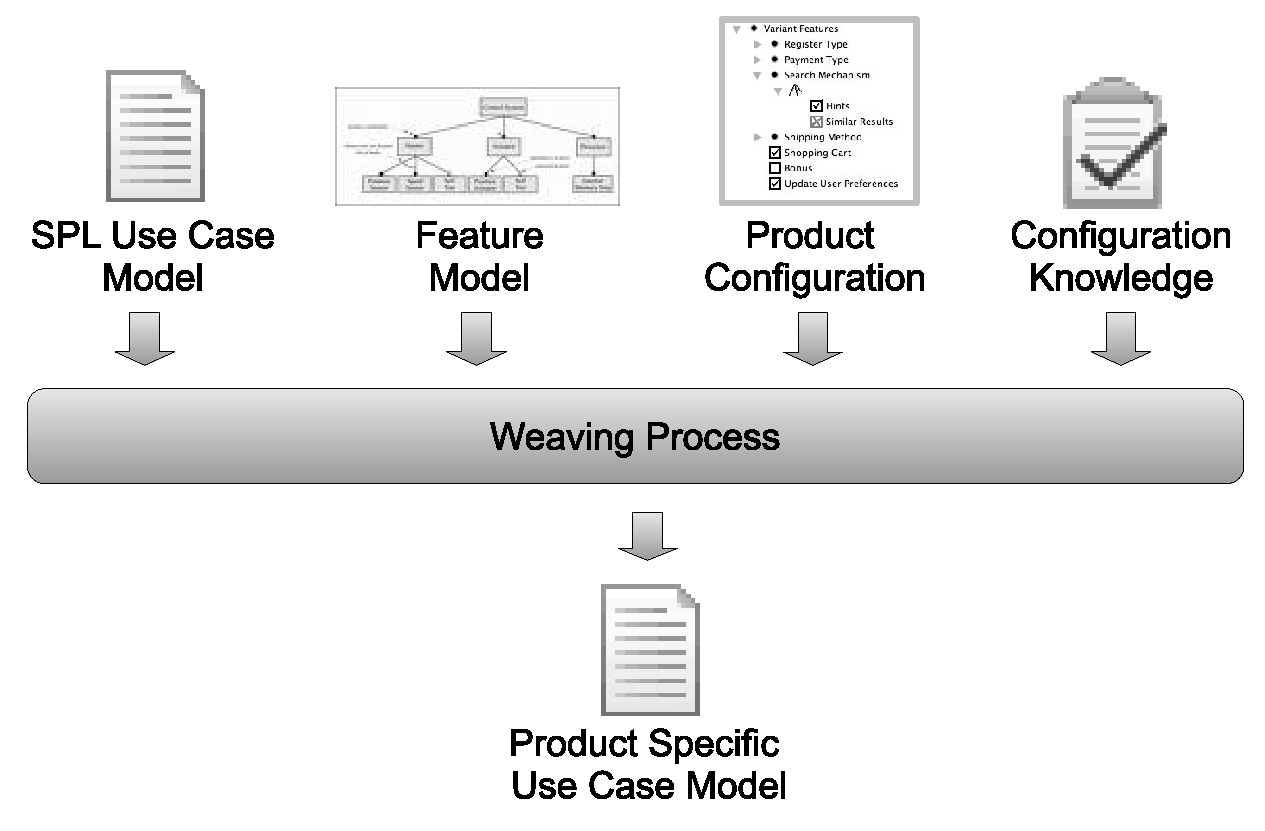
\includegraphics[scale=0.30]{img/weave-process2.eps}
%   \caption{Overview of our weaving process.}
%   \label{fig:weave-process}
%   \end{center}
% \end{figure}
% 
% Although the semantics of each variability mechanism, expressed as weavers in
% our modeling framework, are described in next sections, here we discuss the
% semantics of the \emph{weaving process} (Figure~\ref{fig:weave-process}). The
% weaving process is responsible for generating a use case model that is specific to the
% product configuration. Therefore, the process takes into account a selection of
% features, which characterizes specific instances of a product line. In this
% process, the contribution of the configuration knowledge is fundamental, since
% it is responsible for relating feature expressions (writeen in propositional
% logic) to individual weavers.
% 
% \begin{figure}[ht]
% \begin{code}
% type ConfigurationKnowledge = [Configuration]
% 
% data Configuration  = Configuration {
%  exp :: FeatureExpression,
%  weavers :: [Weaver] 	
% }
% 
% type Weaver = (SPL -> SPLMember) -> SPLMember
% 
% weavingProcess spl fm pc ck =
%    stepRefinement [(w spl) | w <- ws] p
%    where
%     ws = concat [weavers c| c <- ck, eval pc (exp c)]
%     p = (emptyInstance spl fc)
%     stepRefinement l m = ...   	
% \end{code}
% \caption{Weaving Process' interpreter}
% \label{fig:wp-semantics}
% \end{figure}
% 
% Figure ~\ref{fig:wp-semantics} shows our proposed configuration knowledge,
% represented as a list of the algebraic data type $(exp,\ weavers)$, and a valid
% interpreter for the weaving process. Basically,
% the interpreter evaluates a list of weavers ($ws$) that must be applied for
% the specific product configuration. In order to filter the list of weavers, it
% is necessary to verify  ($eval\ pc\ (exp\ c)$) which expressions ($exp\ c$) in
% the configuration knowledge are valid for a specific product configuration
% ($pc$).
% 
% Each weaver is a function that takes as input a SPL model
% ($spl$) and a SPL member ($p$); and returns a refined
% version of the SPL member. At the begining, the SPL member is empty.
% The $stepRefinement$ function composes the sequence of weavers that must
% be applied. Therefore, supposing $ws = [h,g,f]$, the semantics of
% this hypothetical product would be given by:
% 
% \begin{center}
% $ p\ =\ f\ (spl,\ g\ (spl,\ h\ (spl,\ emptyProduct)))  $
% \end{center}
% 
% The next Section presents examples of each input model. All examples were
% extracted from the \emph{eShop} Product Line (briefly introduced in
% Section~\ref{sec:problem}).

%==============================================================
%==============================================================

As mentioned before, the semantic of crosscutting, used for representing our variability management weaving process, is based on the Masuhara and Kiczales work~\cite{kiczales-ecoop-2003}.

First of all, their requirement for characterizing a mechanism as crosscutting is fulfilled by our approach, since different specifications contribute to the definition of a specific SPL member. As a consequence, due to its crosscutting nature, the modeling framework proposed in~\cite{kiczales-ecoop-2003}  is suitable for formalizing variability management compositions.

For simplicity, our weaving process is formally described as being composed by three major weavers: \emph{product derivation weaver}, \emph{scenario composition weaver}, and \emph{bind parameters weaver}. As a customization of MK work, our modeling framework represents each weaver as an 6-tuple (Eq.~\ref{eq:tuple} and Table~\ref{tab:tup-01}), highlighting the contribution of each input language in the composition processes.

\begin{equation}
W = \{o, o_{jp}, L, L_{id}, L_{eff}, L_{mod}\},
\label{eq:tuple}
\end{equation}

\begin{table}[h]
\begin{center}
\caption{Modeling framework elements.} \label{tab:tup-01}
\begin{tabular}{||p{0.6in}||p{2.4in}||}
  \hline
  {\bf Element} & {\bf Description} \\
   \hline
  $o$              & Output language used for describing the results of the weaving process \\ \hline
  $o_{jp}$       & Set of join points in the output language \\ \hline
  $L$              & Set of languages used for describing the input specifications \\ \hline
  $L_{ID}(l)$      & Set of constructions in each input language $l$, used for identifying the output join points \\ \hline
  $L_{EFF}(l)$   & For each input language $l$, this element represent the effect of its constructions in the weaving process \\ \hline
  $L_{MOD}(l)$  & Set of modular unities of each input language $l$\\ \hline
  \hline
\end{tabular}
\end{center}
\end{table}

We represent each weaver by
filling in the seven parameters of our 6-tuple representation, and by stating
how elements of the weaver implementation correspond to elements of the model.

% ---
% Product derivation weaver
% ---
\subsubsection{Product derivation weaver}\label{sub:pd-weaver}

This weaver is responsible for selecting artifacts based on specific product configurations.
As a consequence, it implements the first two activities of our variability management approach:
validating a product configuration against  a feature model and selecting a subset of the SPL assets.
Although in this paper we are focusing only in the selection of scenarios that should be assembled in specific instances
of the SPL, this weaver can be easily extended for managing variabilities in other kinds of assets (aiming at selecting design elements, source components, and test cases).

For instance, applying this weaver for combining the eShop use case model, feature model , and configuration knowledge with the configuration depicted in right side of Figure~\ref{fig:product-config-01-02} will result in the selection of  \emph{Buy Products with Cart}, \emph{Proceed to Purchase}, \emph{Search for Products}, ann \emph{Register User Preferences} scenarios.
 This weaver is implemented by the function \emph{pdWeaver} (Listing~\ref{lst:configure}) and takes as input
a \emph{SPL use case model} (UCM), a \emph{feature model} (FM), a \emph{product configuration} (PC), and a \emph{configuration knowledge} (CK).

Initially, this function verifies if the product configuration is a well formed instance of the feature model (\emph{validInstance} function) --- if it is not the case,  an \emph{InvalidProduct} error is thrown. Then, the IDs of selected scenarios are computed by the \emph{configure} function. This is done by evaluating which feature expressions, defined in the list elements (x:xs) of configuration knowledge, are valid for the specific product instance (\emph{eval} function). Finally, given the resulting list of scenario IDs, the function \emph{retrieveArtifacts} returns the product specific scenarios.
As a consequence, we can realize two levels of crosscutting in this weaver. First, the feature model, the product configuration, and the configuration knowledge crosscut each other in order to contribute to the list of valid scenario IDs composition. Then, the resulting list of scenario IDs crosscuts with the use case model for selecting the product specific scenarios.

\begin{lstlisting}[belowskip=20pt,frame=tb,caption={Product derivation weaver function},label=lst:configure]
pdWeaver :: UCM -> FM -> PC -> CK -> ScenarioList
pdWeaver ucm fm pc ck =
 if not (validInstance fm pc)
 then error InvalidProduct
 else retrieveScenarios ucm (configure pc ck)

configure :: PC -> CK -> ListOfScenarioId
configure pc (CK []) = []
configure pc (CK (x:xs)) =
 if (eval pc (expression x))
  then (artifacts x) ++ (configure pc (CK xs))
  else configure pc (CK xs)
\end{lstlisting}

The model of the \emph{Product Derivation Waver},
in terms of the framework, is showed in Table~\ref{tab:pd-weaver}. The \emph{pdWeaver} function is used to argue that the model is realizable and appropriate~\cite{kiczales-ecoop-2003}. We achieve this by matching the model elements
to corresponding parameters and auxiliary functions in the implementation code. Therefore, the input languages UCM, FM, CK, and PC are represented as different parameters
of the \emph{pdWeaver} function. An instance of the UCM corresponds to the specification of all
SPL scenarios. A FM instance is only responsible for declaring the SPL features and the relationships between
them; as a consequence, there is no coupling between FMs and UCMs. Instead, relationships between features and artifacts are documented in the configuration knowledge. Finally, the PC specifies which features were selected
for a specific product.

\begin{table}[htb]
\begin{center}
\caption{Model of Product Derivation} \label{tab:pd-weaver}
\begin{tabular}{p{0.6in}p{2.4in}}
   \hline\noalign{\smallskip}
  {\bf Element} & {\bf Description} \\
   \noalign{\smallskip}
   \hline
   \noalign{\smallskip}
   $o$               & Product specific scenarios (list of scenarios) \\
   $o_{jp}$        & Scenario declarations \\
   $L$               & \{UCM, FM, CK, PC\} \\
   $UCM_{ID}$ & SPL scenarios \\
   $FM_{ID}$    & SPL features \\
   $CK_{ID}$    & Feature expressions and scenario IDs\\
   $PC_{ID}$    & Product specific feature selection \\
   $UCM_{EFF}$ & Provides declaration of scenarios \\
   $FM_{EFF}$    & Checks if a SPL instance is well formed \\
   $CK_{EFF}$    & Identifies selected artifacts  \\
   $PC_{EFF}$    &Triggers scenario selection \\
   $UCM_{MOD}$ & Scenario \\
   $FM_{MOD}$   & Feature \\
   $CK_{MOD}$    & Each pair $(feature\ expression, artifact\ list)$  \\
   $PC_{MOD}$    & Feature \\
  \hline
  \end{tabular}
\end{center}
\end{table}

The UCM has a greater importance over the other input languages ($UCM_{EFF}$), since it declares the parts that compose the product specific scenarios (the
output of this weaver process generated by the \emph{pdWeaver} function). These scenarios ($UCM_{ID}$) are used in the \emph{retriveScenarios} function in order to identify which artifacts will be assembled in the final product.

In order to identify which artifacts are required for a specific product, the \emph{configure} function ($CK_{EFF}$) checks the feature expression ($CK_{ID}$) against the product specific features ($PC_{ID}$). The effect of FM in this weaver ($FM_{EFF}$) is to check if the PC is well formed. Such evaluation is implemented by the \emph{validInstance} function and considers the PC feature selection ($PC_{EFF}$).


% ---
% Scenario composition weaver
% ---

\subsubsection{Scenario composition weaver}\label{sub:sc-weaver}

This weaver is responsible for the third activity of our variability management
approach. It aims at composing variant scenarios of a use case and is applied whenever a use case scenario supports different execution paths.
This mechanism takes as input the product specific use case model (a list of scenarios). Each scenario, often partially specified, is then composed in order to generate concrete specifications.

As shown in Section~\ref{sub:running}, a variant scenario
might refer to steps either in basic or other variant scenarios. In order
to compute the complete paths defined by a scenario, we need to compose the events that precede all steps referenced by its \emph{From step
clause} (up to the IDLE step), followed by its own steps, and then by all
events that follow all of the steps referenced by its \emph{To step clause} (down to the END step).

For instance, consider a product configured with the features \emph{Shopping Cart} and \emph{Bonus}, which requires the \emph{Buy Products with Cart} scenario, and with the feature \emph{Update User Preferences}. Referring to Figure~\ref{fig:buy-product-changing-flow}, the  \emph{Buy Product with Cart} scenario starts from the IDLE state (\emph{From step} clause) and then, after its own flow of events, goes to Step P1 of \emph{Proceed to Purchase} (see the \emph{To step} clause). In a similar way, Figure~\ref{fig:register-preferences-flow} depicts that \emph{Register User Preferences} scenario starts from any step that is marked with the \emph{RegisterPreferences} annotation (for example, Step P3 of of \emph{Proceed to Purchase}). In this context, the result of applying the composition scenario weaver is a concrete path of execution for this configuration, that can be represented as this sequence of step ids: \mbox{<IDLE, V1, V2, P1, P2.ShipMethod, P3, R1, END>}.

Note that this sequence still has  the \emph{ShipMethod} parameter,
referred in Step P2 of \emph{Proceed to Purchase} scenario. The \emph{Binding parameter weaver}, discussed in next section, is responsible for resolving parameters in the final
product specification.

%Before formalizing the \emph{Scenario composition weaver}  in terms of our modeling framework, we
%first discuss about the abstract representation of scenarios (Listing~\ref{lst:ucm}). We omit elements of the use case model abstract syntax that are not required for understanding this weaver. A scenario has an id, a
%description, a \emph{From step clause} (a list of references for
%existing steps), a list of steps, and a \emph{To step clause} (also
%a list of references for existing steps). A step has an id, a
%specification in the form of a tuple
%(user-action x sytem-response), and a list of annotations
%that can be used to semantically identify the step (avoiding
%fragile pointcuts). Finally, a reference to a step can be either a reference to a \emph{step id} or to a \emph{step annotation}.

%\begin{lstlisting}[belowskip=10pt,frame=tb,caption={Abstract syntax of scenario artifact},label=lst:ucm]
%data Scenario = Scenario id FromStep StepList ToStep
%data Step = Step Id Action Response Annotations
%\end{lstlisting}

The \emph{Scenario Composition Weaver} is implemented by the \emph{scWeaver} function (Listing~\ref{lst:trace}), which takes
as input the product specific use case model (a list of scenarios computed by the previous weaver).
The \emph{scWeaver} function computes the complete paths of each
scenario by calling, recursively, the \emph{completePaths} function. This
function (lines 5-6 in Listing~\ref{lst:trace})
takes as input the product specific use case model (\emph{ucm}) and a specific
scenario (\emph{scn});
and returns all complete paths (a list of \emph{step lists}) of
\emph{scn}. The function \emph{fromList} (called at line 7) is used to
compose all complete paths extracted from the \emph{From step
clause}. In a similar way, the function \emph{toList} (called at
line 7) is used to compose all complete paths extracted from the
\emph{To step clause}. The \emph{match} function (also called at
line 7), retrieves all the steps in \emph{ucm} that satisfy all
\emph{step references} in \emph{From step} or \emph{To step}
clauses.

%Currently, this matching is based on the \emph{step id} (a
%syntactically reference) or on the list of \emph{step annotations}
%(a semantic reference). The ``+++'' operator denotes distributed
%list concatenation.

% \begin{figure*}
% \begin{lstlisting}[belowskip=10pt,frame=tb,caption={Scenario composition weaver function},label=lst:trace]
% scWeaver :: ScenarioList -> [StepList]
% scWeaver scenarioList = [completePaths scenarioList s | s <- scenarioList]
%
% completePaths :: ScenarioList -> Scenario -> [StepList]
% completePaths ucm scn =
%  (fromList ucm (match ucm (fromSteps scn)) +++ [stepsOf scn]) +++  (toList ucm (match ucm (toSteps scn)))
%
% traceModel [] = [[]]
% traceModel (x:xs) = [] : (x) ^ (traceModel (xs))
% \end{lstlisting}
% \end{figure*}

The model of this weaver is in Table~\ref{tab:sc-weaver}. The output ($o$ element of our modeling framework) is the complete paths of the product specific scenarios, computed directly from \emph{scWeaver} function. Therefore, the input language (L) corresponds to the product specific scenarios, related to the \emph{scWeaver}
 parameters.
The join points are modeled as the final scenarios and steps in the output language. They result from the composition of partial scenarios by means of
\emph{from steps} and \emph{to steps} clauses ($L_{ID}$).
The effect of the input languages ($L_{EFF}$) in the composition process is to combine
product specific scenarios that, before this activity, did not define a concrete flow of events. As a consequence, the \emph{match} function
plays a fundamental role in this process, retrieving the steps in the use case model that satisfies the \emph{From step} and \emph{To step} clauses.

\begin{table}[hbt]
\begin{center}
\caption{Model of Scenario Composition Weaver} \label{tab:sc-weaver}
\begin{tabular}{p{0.4in}p{2.6in}}
   \hline\noalign{\smallskip}
  {\bf Element} & {\bf Description} \\
   \noalign{\smallskip}
   \hline
   \noalign{\smallskip}
   $o$               & List of composed scenarios  \\
   $o_{jp}$        & Scenarios and steps of scenarios \\
   $L$               & \{Product specific scenarios (list of scenarios)\} \\
   $L_{ID}$       & From step and to step clauses \\
   $L_{EFF}$    & Defines abstract scenarios  \\
   $L_{MOD}$  &  Scenarios \\
  \hline
  \end{tabular}
\end{center}
\end{table}


After computing the complete paths (using the \emph{scWeaver} function), it is possible to derive another representation for product specific scenarios. This is essentially a \emph{trace model}, since it describe all possible sequences of events specified by the complete paths. This representation is useful for checking, for example, if a non-expected sequence of events is present in a final product, which means that a problem in the composition has occurred. Actually, we used this representation in the verification process of our model (Section~\ref{sub:model-verification}. The \emph{traceModel} function (lines 8 and 9 of Listing~\ref{lst:trace}) is responsible for computing this representation. For instance, the trace model for the the first configuration of our running example is the set of sequences:

\begin{small}
\begin{tabular}{rlc}
$Trace_{C1}$ = & \{<>, <idle>, <idle, S1>, <idle, S1, S2>, \\
                    & <idle, S1, S2, S3>,  <idle, S1, S2, S3, end>, \\
                    & <idle, B1>, <idle, B1, B2>, \ldots, \\
                    & <idle, B1, B2, P1, P2.ShipMethod, P3, end> \}
\end{tabular}
\end{small}


% ---
% Bind parameters weaver
% ---

\subsubsection{Bind parameters weaver}\label{sub:bind-weaver}

This weaver is responsible for the third activity of our variability
management process. Parameters are used in scenario specifications
in order to create reusable requirements. This kind of variability can be applied
whenever two or more scenarios share the same behavior (the sequence
of actions) and differ in relation only to values of a same concept.
For instance, Figure~\ref{fig:proceed-to-checkout} depicts the \emph{Proceed to Purchase}
scenario that can be reused for different \emph{ship methods}. Without this
parameterized specification, and aiming, for example, at automatically generating a test case suite
with a good coverage, it would be necessary to create a specification for each kind of ship method.

This weaver takes into consideration \emph{scenario specifications} and
\emph{product configurations}, which defines the domain values of a
parameter. Thus, in order to reduce the coupling between scenarios and features,
we propose a mapping that relate them. A constraint must be obeyed in this mapping: features related to parameters must be either an {\bf alternative feature} or an {\bf or feature}~\cite{gheyi-alloy-06,czarnecki-wsfactory-2005,czarnecki-book}.

The implementation of this weaver consists of calls to
the \emph{bpWeaver} function (Listing~\ref{lst:bind}) for each step
available in the product specific scenarios or complete paths. This
function (lines 1-5 of Listing~\ref{lst:bind}) takes as
input a mapping (\emph{m}), which relates a scenario parameter to a
feature; a product configuration (\emph{pc}), which defines
the domain values of parameters (expressed as the feature selection); and a step (\emph{s}) that may be parameterized. Then, it replaces all parameters
from \emph{s}, returning it as a suitable representation with the
corresponding parameter values. Each text between the symbols ``$<$'' and ``$>$''
(defined in the user action or system response of a
step) is treated as a parameter and must be defined in the
mapping.

For example, if a product is configured with either \emph{Economical} and
\emph{Fast} ship methods, the result of applying this weaver for
the Step P2 of the \emph{Proceed to Purchase} scenario will result in the
representation (\emph{Economical or Fast}) in each place that the parameter \emph{ShipMethod} is referred.

Table~\ref{tab:bp-weaver} describes the Bind Parameters model. This weaver just resolves parameters in scenario specifications. Therefore, its output language is also a list of scenarios; but with resolved parameters (the join points).

\begin{lstlisting}[belowskip=10pt,frame=tb,caption={Bind parameter weaver function},label=lst:bind]
bpWeaver :: Mapping -> PC -> Step -> Step
bpWeaver m pc s =
 if (length (extractParameters (s)) == 0)
  then s
  else replaceParameterValues m pc s
\end{lstlisting}


\begin{table}[th]
\begin{center}
\caption{Model of Bind Parameters Weaver} \label{tab:bp-weaver}
\begin{tabular}{p{0.7in}p{2.3in}}
   \hline\noalign{\smallskip}
  {\bf Element} & {\bf Description} \\
   \noalign{\smallskip}
   \hline
   \noalign{\smallskip}
   $o$               & List of scenarios with resolved parameters  \\
   $o_{jp}$        & Each resolved parameter \\
   $L$               & \{UCM, PC, Mapping\} \\
   $UCM_{ID}$ & Parameterized steps \\
   $PC_{ID}$    & Selected features related to parameters \\
   $Mapping_{ID}$ & Key entries (parameter name) of the mapping\\
   $UCM_{EFF}$ & Declares parameterized scenarios \\
   $PC_{EFF}$    & Defines the domain value of parameters \\
   $Mapping_{EFF}$ & Relates parameters to features \\
   $UCM_{MOD}$ & Use case scenarios \\
   $PC_{MOD}$    & Selected features \\
   $Mapping_{EFF}$ & Each entry in the mapping \\
  \hline
  \end{tabular}
\end{center}
\end{table}

The use case model (UCM) defines the list of scenarios that might be parameterized ($UCM_{EFF}$). Each step of a scenario ($UCM_{ID}$), indeed, contributes to the definition of one join point in this weaver. The
other contributions come from the configuration knowledge (CK), in the sense that the domain values
of a parameter is defined ($CK_{EFF}$) in the product specific features; and from the mapping ($m$ parameter of the \emph{bind} function) that is used for relating parameters to features.
In what follows, we discuss about some verifications applied to the weaving processes just presented. Such verifications were conduced by applying both \emph{random} and \emph{guided} test cases.

In the next section we present an evaluation of our approach based on the
specification of SPLs in different domains.

% \subsection{Model Verification}\label{sub:model-verification}
%
% The specifications presented in the
% previous section allow us to verify if the composition
% processes have desired properties or behavior.
% Aiming at doing that, we applied two techniques for testing
% Haskell programs: unit tests; and
% formal specifications for checking properties of our modeling
% framework.
%
% Unit tests were developed using the HUnit library~\cite{hunit-tutorial}.
% Similar to other \emph{xUnit} tools, it requires well defined input data and
% expected results. After that, it is possible to check if
% a call to a \emph{function under test}, sending the previous defined input data as
% argument, yields a value equal to the expected results.
% For instance, we applied unit tests for checking if the composition process
% for the product configurations depicted in Figure~\ref{fig:product-config-01-02}
% yields expected traces. Therefore, the trace model notation discussed in
% a previous section plays an important role in our verification process.
% In order to perform such kind of checking, we first implemented
% a \emph{refine} function (Listing~\ref{lst:traceRefinement}),
% which checks if all sequences of traces in the \emph{model under test} (mut) are
% present in the expected results --- named here as reference model.
%
% % \begin{lstlisting}[belowskip=10pt,frame=tb,caption={The \emph{traceRefinement} function},label=lst:traceRefinement]
% % refine :: TraceModel -> TraceModel -> Bool
% % refine referenceModel mut =
% %  and [exists (x referenceModel) | x <- mut]
% % \end{lstlisting}
%
% Then, we defined expected traces (such as \emph{data01} and
% \emph{data02} in Listing~\ref{lst:unitTest}) for both configurations
% of Figure~\ref{fig:product-config-01-02}, considering the complete paths
% showed in Figure~\ref{fig:complete-paths}. Additionally, two trace models
% (\emph{tm01} and \emph{tm02}), computed by the composition process, were defined
% as input data. Notice that the input trace models were computed varying just the
% products configurations (\emph{pc01} and \emph{pc02}).
% Finally, test cases (such as tc01 and tc04) were developed
% for verifying expected and non-expected traces in the resulting composed models.
%
% \begin{lstlisting}[belowskip=10pt,frame=tb,caption={Unit test for composition process},label=lst:unitTest]
% data01 = [[], [idle], [idle, 1M], ...
%  [idle,1M, 2M, 3M, 4M, 5M, end]]
%
% data02 = [[],[idle], [idle, V1], ...
%  [idle, V1, V2, 3M, 4M, 5M, end]]
%
% tm01 = computeTraces (fm01 pc01 ck01 ucm01)
% tm02 = computeTraces (fm01 pc02 ck01 ucm01)
% -- expected traces for configuration 01
% tc01 =
%  TestCase (assertBool (refine tm01 data01 tm01))
%
% -- non-expected traces for configuration 02
% tc04 =
%  TestCase (assertBool (not (refine data01 tm02)))
% \end{lstlisting}
%
% Based on the examples just presented, unit tests are useful for
% verifying the presence of errors under well defined test cases
% (described by the input data and expected results). A complementary
% approach consists in checking function properties based on formal
% specifications. In order to perform this kind of verification, we use
% the \emph{QuickCheck} library~\cite{claessen00-icfp-2000}, which provides
% an \emph{embedded specific language} that is used to specify
% properties of Haskell programs; and several functions for checking
% formal properties and for randomly generating input data.
% This second verification approach is also suitable in our context since
% several properties related to each input model (or to the compositions between them)
% should be obeyed. Applying just unit tests for checking these properties may
% require a huge effort for designing and implementing input data and expected results
% for each interesting test scenario. On the other hand, this formal technique
% requires the specification of properties that a \emph{function under test}
% should hold. These properties are then checked against randomly input data.
%
% %It is important
% %to notice that functions for generating input data can be overloaded in the \emph{QuickCheck}
% %library, which means that we can define the generation of data based on occurrence probabilities.
%
% We applied this verification technique for checking several properties of feature modeling (briefly introduced in Section~\ref{sec:problem}). For example, an alternative feature requires exactly one sub feature to be selected in a product configuration. Using the \emph{QuickCheck} library, this property can be expressed as the function \emph{prop\_ExactlyOneSelected} in Listing~\ref{lst:quick-check}.
% It takes two feature as parameters and returns a property to be checked. The first parameter (fm) should be an alternative feature (from a feature model). The second one (fc), instead, is a corresponding feature from the product configuration. If the number of children of \emph{fc} is different than one (the expression before the implies symbol), it is expected that a call to the \emph{existError} function will return \emph{True}. After specifying this kind of property, it is possible to verify if they hold for different input data.
%
% \begin{figure*}
%  \begin{lstlisting}[belowskip=10pt,frame=tb,caption={Example of QuickCheck property},label=lst:quick-check]
% prop_ExactlyOneSelected :: Feature -> Feature -> QuickCheck.Property
% prop_ExactlyOneSelected fm fc = (not (length (children fc) == 1)) =>
%  existError (checkAlternativeFeature fm fc)
% \end{lstlisting}
% \end{figure*}
%
% We also performed this kind of verification for checking properties related to the weaving process. For instance, we defined properties for checking if all scenario parameters are related exclusively to \emph{alternativeFeatures} or \emph{orFeatures}. Such constraint was discussed in the previous section.
%
% Both verification approaches were important to improve the confidence of our models. Actually, several unit tests and properties revealed to us interesting case; we were not initially concerned with some of them. To our knowledge, no existing work for representing variability management in scenarios apply these level of verifications.
%